
% write Transformation NOT transform
% TODO:
% Consistent usage of characters OR symbols


% Finish citations...

% Finish other TODOs
% 
% Ændrer alle grafer til Matplotlib grafer, OG lav en average hvis der ikke er der
% URLs i reference er i stykker når der er newline
% Skal jeg lave new line mellem sections? Nej
% proof of huffman optimality

% Figure in RLE, show a bar chart like the figure in 10.

% The output will then be the concatenation of ...

% This paper is structured as follows: 1) vs Section 1

% Burrows-Wheeler, should be Burrows--Wheeler

% https://www.cs.cmu.edu/~sleator/papers/adaptive-data-compression.pdf

\documentclass{article}
\usepackage[utf8]{inputenc}
\usepackage{amsmath}

\usepackage{algorithm}
\usepackage{algpseudocode}

\usepackage{biblatex} %Imports biblatex package
\usepackage[dvipsnames]{xcolor}
\usepackage{caption}
\usepackage{float}

\usepackage{tikz}
\usetikzlibrary{shapes.multipart,matrix,positioning}

%%%
\usepackage{listings}
\usepackage{xcolor}

\definecolor{codegreen}{rgb}{0,0.6,0}
\definecolor{codegray}{rgb}{0.5,0.5,0.5}
\definecolor{codepurple}{rgb}{0.58,0,0.82}
\definecolor{backcolour}{rgb}{0.95,0.95,0.92}
\definecolor{Black}{RGB}{0.05,0.05,0.05}	
	\definecolor{brandeisblue}{rgb}{0.0, 0.44, 1.0}

\lstdefinestyle{mystyle}{
    backgroundcolor=\color{backcolour},   
    commentstyle=\color{codegreen},
    keywordstyle=\color{magenta},
    numberstyle=\tiny\color{codegray},
    stringstyle=\color{codepurple},
    basicstyle=\ttfamily\footnotesize,
    breakatwhitespace=false,         
    breaklines=true,                 
    captionpos=b,                    
    keepspaces=true,                 
    numbers=left,                    
    numbersep=5pt,                  
    showspaces=false,                
    showstringspaces=false,
    showtabs=false,
    tabsize=2
}
\usepackage[
            urlcolor  = blue,
            anchorcolor = blue]{hyperref}
\hypersetup{colorlinks=true, linkbordercolor=Black,linkcolor=Black, citecolor=brandeisblue}
\usepackage[capitalize,nameinlink,noabbrev]{cleveref}
\usepackage{tabularx}
\usepackage{setspace}

\lstset{style=mystyle}
%%%%

\addbibresource{biblo.bib} %Import the bibliography file

\begin{document}


\begin{titlepage}
\Large
\renewcommand{\thepage}{Title}
\thispagestyle{empty}
\begin{center}
   \vspace*{1cm}
\linespread{1.25}
       {\doublespacing \Huge \textbf{Lossless File Compression with bzip2}}
\linespread{1}
       \rule{\linewidth}{1pt}
       {\huge Bachelor Thesis \\[1ex]
       \Large Department of Mathematics and Computer Science \\
       University of Southern Denmark}
       
    \vspace*{1cm}
    \large \today
\end{center}
\vspace{4cm}
\Large
\begin{tabularx}{\textwidth}{lXr}
    Author & & Ahmad Mahir Sadaldin Othman\\ 
    & & ahoth19@student.sdu.dk\\ \\
\end{tabularx}
\begin{tabularx}{\textwidth}{lXr}
    Supervisor & & Rolf Fagerberg \\
    & & rolf@imada.sdu.dk \\ \\
\end{tabularx}

\vfill
\centering
\includegraphics[width=0.4\textwidth]{images/sdulogo.png}
\end{titlepage}


\pagenumbering{roman}

\newpage

\begin{abstract}
In this paper we describe the file compressing program \texttt{bzip2} and the techniques it uses to achieve compression. We describe it in relation to the research report published in 1994 by Michael Burrows and David J. Wheeler that laid the groundwork for it. We describe the theory behind Burrows--Wheeler transform, along with the Move-to-front encoding, Run-length encoding, and Huffman encoding using multiple Huffman trees, and how some of these are implemented in \texttt{bzip2}.
The purpose of this paper is to justify the usage of these different algorithms in sequential order, and describe why they tend to work well together in practice.
We have described the reasoning behind using multiple Huffman trees, and the method \texttt{bzip2} uses to initialize them and then improve them over several iterations. We experiment using our implementation of \texttt{bzip2} where we tweak some of these values and techniques in an attempt to understand their role to further be able to improve them. We have experimented by changing hardcoded values in \texttt{bzip2} and given our suggestions on methods that would improve compression ratio performance. We have concluded that the initialization and improvement of these Huffman trees can sometimes reach a local optimum instead of a global optimum, which allows for improvement. 


\end{abstract}

\newpage

\renewcommand{\abstractname}{Dansk resumé}
\begin{abstract}
I denne opgave beskriver vi filkomprimeringsprogrammet \texttt{bzip2} og de teknikker den bruger til komprimering af data. Vi beskriver forskningsrapporten offentliggjort i 1994 af Michael Burrows og David J. Wheeler hvor de introducerede deres nyopdagede reversible datatransformation, nemlig Burrows-Wheeler Transform. De viste nemlig, at deres brug af den bye datatransformation samt Move-to-front indkodningen og Huffman indkodningen samt andre heuristikker gav imponerende kompressionsresultater. Vi undersøger, beskriver og forklarer denne datatransformation i detaljer og dets irreversible natur. Vi beskriver yderligere brugen af Move-to-front indkodningen og Huffman indkodningen efter denne datatransformation og begrunder hvorfor kombinationen af disse teknikker opnår stærke kompressionsresultater. Vi beskriver derefter \texttt{bzip2}, som implementerer disse algoritmer og andre teknikker, herunder de to trin af Run-length indkodningen og dets brug af flere Huffman-træer, hvor hver Huffman træ individuelle dele af dataen. Vi eksperimenterer med vores egen implementation af \texttt{bzip2}, hvor vi justerer værdier i et forsøg på at forstå deres påvirkning og hvordan de kan forbedres. Vi har eksperimenteret med at ændre de hårdkodede værdier i \texttt{bzip2} og præsenteret forslag til metoder, der ville forbedre komprimeringsforholdets ydeevne. Det viser sig, at initialiseringen og forbedringen af Huffman-træerne i visse tilfælde kan nå et lokalt optimum i stedet for et globalt optimum, så der er plads til forbedring.
\end{abstract}

\newpage

\tableofcontents
%\listoffigures
%\listoftables

\newpage
\pagenumbering{arabic}
\section{Introduction}
%Kontekst (hvor er vi henne i datalogien?) \\
%Motivation for problemstillingen \\
%Historik (forskningsresultater, med ref. til litteratur) \\
%I dette projekt vil vi.... (the reader is now in position to understand this, based on the previous three points)

%Indsnævre (movtivation til compression) ind til Burrow Wheeler transform og bzip2, og så dette projekt vil vi....
%komprimerings faktor? 

% There is a higher demand for storing data than ever before
The evolution of data storage has been through rapid development the past few decades. Going from the preliminary commercial floppy disks containing a mere 80 kB of data to the 3-½ inched IBM disks of 1.44 MB. Back then, it could be hard to imagine a need for more space than that. Today, however, installing Microsoft Office on Windows uses 4 GB of disk space, which would require 2778 of these 3-½ inched floppy disk. It is clear, that our need for information and data is increasing with time.
This has given rise to the field of data compression, which aims to better utilize storage capacity by reducing the size of the file and therefore also reducing the transmission time.

The field of data compressing can be split into two categories: lossy and lossless. Lossy data compressors generate an encoded file that when decompressed only output an approximation of the original file, resulting in data loss. This is mostly used for media-type formats like images, videos, and audio files, where data loss is acceptable, and is a trade-off to achieve better compression ratios (the ratio between the compressed file and the original file). % is unnoticeable to the user but can allow for better compression.
% They do not guarantee the decompressed file to match the original file exactly but can accept some percentages of error, where that percentage is usually implemented to be optional to the user. 
Notable lossy compressing programs include the image compressor \texttt{JPEG} \cite{jpeg1}, audio and video compressors \texttt{MPEG} \cite{mpeg1}\cite{mpeg2}.
% TODO: Er optional in terms of error vs.
For lossless compressors, the requirement is that the original file can be fully recovered after decompression with no loss or ambiguity. This type of compression is used for a wider range of data, including text documents, DNA, and source code. All these require the entire file to be recoverable since even small deviations in the data can be unacceptable.
Notable lossless compressors belong to the dominant class of Lempel-Ziv \cite{ziv1977universal} based compressors, which include \texttt{zip}, \texttt{gzip}, \texttt{lzma} \cite{lzmaformat} and \texttt{zstd}. % Another class, which is relatively newer, is the Burrows--Wheeler based compressors, including 
% TODO: TODO: skal det her være der Det ovenover.?
% Compressors input a file and output an encoded file. This encoded file is generally shorter than the input file but contains enough information so that a decompressor can regenerate the original file from the encoded file. Compressors can do this by removing redundant information in the data. % Er det her trivielt?


When deciding which algorithm to use for lossless compression there are three major factors to consider, the trade-off between compression ratio, compression- and decompression speed. % This is why there are many different possible methods. Pareto frontier/efficiency
For some purposes, we might want to compress fast but still with a relatively good compression ratio, while other times compression ratio may be the main focus. This trade-off gives a Pareto-frontier for compressors, where two compressors in the Pareto-front are non-comparable since they depend on the use case of the user.
One program that is one of the champions of compression, which frequently lies on the Pareto-frontier is \texttt{bzip2} \cite{bzip2homepage} \cite{bzip2gitlab} \cite{bzip2formatspecification}. It generally achieves a better compression ratio than both \texttt{zip} and \texttt{gzip} with the trade-off of having worse results in both compression- and decompression time \cite{gzipzipbzip2}. \texttt{bzip2} also competes with the 7zip default compressor \texttt{lzma}. The \texttt{bzip2} compressor generally has a worse compression ratio and decompression time, but achieves better results in terms of compression time \cite{gzipbzip2lzma}.

% TODO: Nævn burrows wheeler transform, og hvilke BWT der stammer fra den

\texttt{bzip2} is a lossless general-purpose compression program developed and released in 1996 by Julian Seward and later maintained by Mark Wielaard, Micah Snyder, and Federico Mena. % TODO: Verify authors and current maintainers
The compressor was developed from the result of a research report titled \texttt{A Block-sorting Lossless Data Compression Algorithm} which was released in 1994 by Michael Burrows and David J. Wheeler \cite{bwt1} \cite{manzini1999burrows}.
Burrows and Wheeler introduced a previously undiscovered reversible data transformation, now known as the Burrows--Wheeler Transform (\texttt{BWT}), which, followed by Move-to-front (\(\texttt{MTF}\)) encoding \cite{bentley1986locally} and Huffman encoding \cite{huffman1952method} achieves good compression results.
\texttt{bzip2} combines these three algorithms, along with some other compression techniques and algorithms to achieve its compression results.
% This has led to a bunch of variants and a bunch of compressors

In this paper, we describe the \texttt{bzip2} compressor in terms of the individual algorithms that it consists of. 
We explore the original research report that laid the groundwork for the \texttt{bzip2} and examine the core reversible data transformation, that the research report introduces. 
We examine the algorithms used in \texttt{bzip2} and analyze their role and contribution to compressing the data.

This paper is structured as follows. In \cref{sec:TABW} we describe the core transform in the \texttt{bzip2} compressor by examining the paper describing it. Here we look at how to compute the transform efficiently and how it can be reversed. We also describe the follow-up compression techniques that were recommended in the paper by Burrows and Wheeler after the \texttt{BWT}, which \texttt{bzip2} also uses. In \cref{sec:BZIP2} we examine \texttt{bzip2} and introduce the additional compression techniques that are used in \texttt{bzip2}. Here we also examine the implementation of these different algorithms in the compressor. Lastly in \cref{sec:EXPERIMENTS} we analyze different results with our custom parameters for the algorithms used. Our analysis is in terms of the compression ratio on the Silesia Corpus \cite{silesiaCorpus}.


\section{The Algorithm of Burrows and Wheeler}\label{sec:TABW}
On May 10. 1994, Michael Burrows and David J. Wheeler released a research report titled \texttt{A Block-sorting Lossless Data Compression Algorithm}. In this report, they described a previously unseen reversible data transformation that was previously discovered by Wheeler but unpublished. The data transformation, now known as the Burrows--Wheeler Transform (\texttt{BWT}) has the property of re-ordering the string so that similar characters appear together in runs.
Burrows and Wheeler showed that this property of the \texttt{BWT}, allows the data to be efficiently compressed using other "simple" algorithms.

The algorithm in the report first transforms the data using \texttt{BWT}, it then encodes it using Move-to-front encoding, and then using Huffman encoding along with a Run-  encoding-like implementation. We will describe the first three of these data transformations separately in the following sections.

\subsection{Burrows--Wheeler Transform}
% TODO: First discovered by Wheeler, but not released due to non-practical way of calculating it, they then worked together until they found a good way
(\texttt{BWT}) is a reversible data transform that re-orders the string, creating a permutation of it that is generally more compressible. The transform is itself not a compressor but is used as a data compression pre-processor since it has the tendency, for human-readable data, to group similar characters up in runs, as we will show in \cref{sectionBWTEffectOnData}.

Given an input string \(S\), \texttt{BWT} outputs a permutation \(L\) and a number \(I\). Burrows and Wheeler showed how given \(L\) and \(I\), we can reconstruct the original string \(S\). 

\subsubsection{Transform}
The transform is computed conceptually by constructing a matrix where each row is a cyclic shift of the string \(S\) (including \(S\) itself) and then sorting the rows lexicographically. The output will then be the concatenation of the characters appearing last in the strings in the row-sorted matrix.

To illustrate this we give an example of computing the \texttt{BWT} of the string \(S = 'abracadabra'\).

\begin{figure}[H]
    \[
        \begin{tabular}{|c|c|}
            \hline
            0 & abracadabra \\ \hline
            1 & bracadabraa \\ \hline
            2 & racadabraab \\ \hline
            3 & acadabraabr \\ \hline
            4 & cadabraabra \\ \hline
            5 & adabraabrac \\ \hline
            6 & dabraabraca \\ \hline
            7 & abraabracad \\ \hline
            8 & braabracada \\ \hline
            9 & raabracadab \\ \hline
            10 & aabracadabr \\ \hline
        \end{tabular}
        \qquad \longrightarrow \qquad
        \begin{tabular}{|c|c|}
            \hline
            10 & aabracadabr \\ \hline
            7 & abraabracad \\ \hline
            0 & abracadabra \\ \hline
            3 & acadabraabr \\ \hline
            5 & adabraabrac \\ \hline
            8 & braabracada \\ \hline
            1 & bracadabraa \\ \hline
            4 & cadabraabra \\ \hline
            6 & dabraabraca \\ \hline
            9 & raabracadab \\ \hline
            2 & racadabraab \\ \hline
        \end{tabular}
    \]
    \captionof{figure}{The cyclic shifts of \(S\) (left) sorted lexicographically (right). The output is then the concatenation of the last character in each string of the sorted row-matrix \(L = "rdarcaaaabb"\) and the row number of the original string \(S\) in the sorted cyclic shifts matrix \(I = 2\).}
\end{figure}
We observe the effect this transform had on the input string \(S="abracadabra"\) which contained zero runs of identical characters. The output string \(L="rdarcaaaabb"\) however has two runs, the first containing 4 \(a\)'s, and the second containing 2 \(b\)'s.
Since we have defined each row in the matrix to be a cyclic shift of our original string, then obviously, in the unsorted matrix each row and column is a cyclic shift of \(S\). After sorting the rows of the matrix, the rows remain cyclic shifts but the columns will no longer necessarily be the cyclic shifts of \(S\) but they will remain a permutation of it. % TODO format sentence better?
This algorithm provides a good conceptual way to imagine and explain the \texttt{BWT} but is not used in practice since it requires constructing the entire matrix in memory, requiring \(O(n^2)\) space for input of size \(n\).

\subsubsection{Transform from Suffix Arrays} % Should this be here?
A more efficient implementation, and how the transform is computed in practice is by observing that the problem of sorting the cyclic shifts of a given string, can be reduced to computing the suffix array of the string. 

Given the same string as previously \(S="abracadabra"\) that we wish to transform. We introduce a new character \(\$\) to \(S\) and append it to the end of the string. \(\$\) is a character that does not previously appear in \(S\) and is lexicographically the smallest character. This gives us \(S' = "abracadabra\$"\). We can repeat the same procedure to compute the \texttt{BWT} as explained previously.
\begin{figure}[H]
    \[
        \begin{tabular}{|c|c|}
            \hline
            0 & abracadabra\$ \\ \hline
            1 & bracadabra\$a \\ \hline
            2 & racadabra\$ab \\ \hline
            3 & acadabra\$abr \\ \hline
            4 & cadabra\$abra \\ \hline
            5 & adabra\$abrac \\ \hline
            6 & dabra\$abraca \\ \hline
            7 & abra\$abracad \\ \hline
            8 & bra\$abracada \\ \hline
            9 & ra\$abracadab \\ \hline
            10 & a\$abracadabr \\ \hline
            11 & \$abracadabra \\ \hline
        \end{tabular}
        \qquad \longrightarrow \qquad
        \begin{tabular}{|c|c|}
            \hline
            11 & \$abracadabra \\ \hline
            10 & a\$abracadabr \\ \hline
            7 & abra\$abracad \\ \hline
            0 & abracadabra\$ \\ \hline
            3 & acadabra\$abr \\ \hline
            5 & adabra\$abrac \\ \hline
            8 & bra\$abracada \\ \hline
            1 & bracadabra\$a \\ \hline
            4 & cadabra\$abra \\ \hline
            6 & dabra\$abraca \\ \hline
            9 & ra\$abracadab \\ \hline
            2 & racadabra\$ab \\ \hline
        \end{tabular}
    \]
    \captionof{figure}{The cyclic shifts of \(S'\) (left) sorted lexicographically (right). The output is again the concatenation of the last character in each string of the sorted cyclic shifts matrix \(L = "ard\$rcaaaabb"\) and the row number of the original string \(S'\) in the sorted cyclic shifts matrix \(I = 3\).}
\end{figure}
% In the lexicographically sorted alphabet \Sigma = $abcd

Since \(\$\) is the smallest character lexicographically when we sort the rows lexicographically, we only need to sort up to and including the \(\$\) symbol. This is also the case when constructing the suffix array of \(S'\). This means that the order the rows end up in, in the sorted rows-matrix of the \texttt{BWT}, is the same order the suffixes are in, in the suffix array. To illustrate this we construct the suffix array \(SA\) of \(S'\)\cite{manber1993suffix} \cite{simpson2010efficient}. 
\begin{figure}[H]
    \begin{equation*}
        \begin{tabular}{|c|l|}
        \hline
        i & \\ \hline
        0 & abracadabra\$ \\ \hline
        1 & bracadabra\$ \\ \hline
        2 & racadabra\$ \\ \hline
        3 & acadabra\$ \\ \hline
        4 & cadabra\$ \\ \hline
        5 & adabra\$ \\ \hline
        6 & dabra\$ \\ \hline
        7 & abra\$ \\ \hline
        8 & bra\$ \\ \hline
        9 & ra\$ \\ \hline
        10 & a\$ \\ \hline
        11 &\$ \\ \hline
        \end{tabular}
        \qquad\longrightarrow\qquad
        \begin{tabular}{|c|c|l|}
        \hline
        i & SA[i] & \\ \hline
        0 & 11 &\$ \\ \hline
        1 & 10 & a\$ \\ \hline
        2 & 7 & abra\$ \\ \hline
        3 & 0 & abracadabra\$ \\ \hline
        4 & 3 & acadabra\$ \\ \hline
        5 & 5 & adabra\$ \\ \hline
        
        6 & 8 & bra\$ \\ \hline
        7 & 1 & bracadabra\$ \\ \hline
        8 & 4 & cadabra\$ \\ \hline
        
        9 & 6 & dabra\$ \\ \hline
        10 & 9 & ra\$ \\ \hline
        11 & 2 & racadabra\$ \\ \hline
        \end{tabular}
    \end{equation*}
    \captionof{figure}{The suffixes of \(S'\) (left) and the Suffix Array \(SA\) of \(S'\) (right)}
\end{figure}
The \texttt{BWT} can then be computed directly from the Suffix Array \(SA\) and our original string \(S\). We build the string \(L\) for each index \(i = 0 \dots |S|-1\):
\[
    L[i] = \begin{cases} 
        S[SA[i] - 1] & SA[i] > 0 \\
        \$ & SA[i] = 0 \\
   \end{cases}
\]
The character in \(L[i]\) will be the character one step left of the character at index \(SA[i]\) in \(S\), which is \(S[SA[i] - 1]\). When \(SA[i] = 0\) the character will be the special \(\$\) character. In the same example we will have the same string \(L = "ard\$rcaaaabb"\) and \(I = 3\).

This reduces the problem of finding the \texttt{BWT} of \(S\) to the problem of constructing the suffix array of \(S\). We note that it is redundant to store both the special character \(\$\) in the string and the value of \(I\), since \(I\) will always be the index of \(\$\) in the transformed string. Since the original string had the special character appended to the end of the string. We can therefore choose to omit \(\$\) from \(L\).

% TODO: How they did it in the paper, counting sort on the first two characters, then quicksort on the ones with the same two first characters

\subsubsection{Effect on Data}\label{sectionBWTEffectOnData}
The location in which a character appears depends entirely on its right context, and how it sorts in comparison to the other characters with a similar right context. This is the case since when sorting the cyclic shifts of a string, characters that contain similar right contexts will be grouped. We consider an example of a large enough English text which may consist of many occurrences of the substring 'the\textvisiblespace'. 
After sorting the cyclic shifts of this text, there will be an interval of rows which are the cyclic shifts starting with the substring 'he\textvisiblespace'. For that, the character to the left of that right context would with reasonable probability be the letter 't'. Although it could also be 's' in case of the substring being 'she\textvisiblespace', or 'c' in case of the substring being 'cache\textvisiblespace'.
The distribution of the characters 't', 's' and 'c' in the case of the right context 'he\textvisiblespace', would then entirely depend on the words following that substring. 

This means that for strings which contain many occurrences of the same substrings, as is generally the case with non-random data, the frequency of different characters that appear with that right context is small.
\begin{center}
    \dots
    TttttTtttttttttTttTts\textvisiblespace ttttt\textvisiblespace ttts\textvisiblespace tttttttttttttttsttttts\textvisiblespace s\textvisiblespace t\textvisiblespace tsttstttstttstttsts \\
    tt\textvisiblespace tt\textvisiblespace tt\textvisiblespace s\textvisiblespace tttttt\textvisiblespace ttstt\textvisiblespace \textbackslash nSss\textvisiblespace Ttssts
    \dots
\end{center}

Example from a substring of the output of the \texttt{BWT} on the last 10000 characters of the file \texttt{dickens} in the Silesia Corpus. The output of the \texttt{BWT} above is limited to the characters whose right context starts with the substring 'he\textvisiblespace'. We note that these are all consecutive as rows in the sorted matrix, and therefore consecutive in the \texttt{BWT} of the text segment. It is noticeable that this segment of the text not only contains many occurrences of the substring 'the\textvisiblespace', but that it also contains occasional occurrences of the substrings 'she\textvisiblespace', '\textvisiblespace he\textvisiblespace', 'Th\textvisiblespace', and one occurrence of '\textbackslash nhe\textvisiblespace' and 'She\textvisiblespace'.
\begin{center}
    \dots
    sssstTttttttttTtttTttttttttttTttTtstst\textvisiblespace tttttt\textvisiblespace \textvisiblespace tttst\textvisiblespace ttttttssttttttttttttttts\textvisiblespace \\
    ttttttssss\textvisiblespace ssss\textvisiblespace ttts\textvisiblespace tttsssttsttsttTtttssttttttsttttttttststtt\textvisiblespace sttttt\textvisiblespace tt\textvisiblespace Sst\textvisiblespace sstttts \\
    tttttt\textvisiblespace ttttstt\textvisiblespace s\textbackslash nSSS\textvisiblespace ssss\textvisiblespace \textvisiblespace Ttsssstst
    \dots
\end{center}
To see the effect on a larger text segment, we approximately double the size of the text segment used previously, to the result of the \texttt{BWT} on the last 20000 characters instead. We again only see the substring of the resulting \texttt{BWT} on the characters with a right-context starting with 'he\textvisiblespace'.
% TODO write some more (even with double the size...)
Even with doubling the size on the input we performed the \texttt{BWT} on, there are no new unique characters in this larger subset than there were previously. This shows the low local character frequency observed from the \texttt{BWT}.
\begin{center}\footnotesize
\dots
ssssttttTttttttttttttTtTTTtTttTtttttttTTtttTTtTTttTTTtTttTtTtttttttttt
ttttTttttttTtttTttttttttttttttttttttttttTtTtttttttttttttttTtttTttttttttttttt
ttttttttttTttTtttTTttttttttTtTtttt\textvisiblespace tstttttt\textvisiblespace Stt\textvisiblespace st\textvisiblespace ssstttT\textvisiblespace st\textvisiblespace tTTtstt\textvisiblespace stt
stt\textvisiblespace tttstTtttttsttttttttttttttS\textvisiblespace ss\textvisiblespace \textvisiblespace sTtTt\textvisiblespace s\textvisiblespace sttttttttttsttttttttttttstttt
tttt\textvisiblespace tttttttttttsttttttts\textvisiblespace \textvisiblespace \textvisiblespace \textvisiblespace s\textvisiblespace s\textvisiblespace \textvisiblespace tttsstttttttttttttttttststsssssssstttttt
tttttttttttttttttssttsttttttttttTtttTttTttt\textvisiblespace tttTttt\textvisiblespace \textvisiblespace \textvisiblespace tTtttttttttttttt\textvisiblespace tt
tttttttttTtttttttt\textvisiblespace \textvisiblespace s\textvisiblespace tt\textvisiblespace ttttTTtttttttTttttt\textvisiblespace ss\textvisiblespace ss\textvisiblespace sSs\textvisiblespace Ss\textvisiblespace s\textbackslash\textvisiblespace n\textvisiblespace sSsss\textbackslash\textvisiblespace n\textbackslash\textvisiblespace n\textvisiblespace \textvisiblespace s\textvisiblespace \textvisiblespace s
\textbackslash\textvisiblespace n\textvisiblespace \textvisiblespace \textbackslash\textvisiblespace n\textvisiblespace s\textvisiblespace ss\textvisiblespace \textvisiblespace Ss\textvisiblespace s\textvisiblespace sttttttttssssss\textvisiblespace ss\textvisiblespace ssSs\textvisiblespace tSttTTtttttttT\textvisiblespace tttttttttTtttTttttt
ttt\textvisiblespace tssSss\textvisiblespace ssstttttsttttst\textvisiblespace Ssssstttttsttt\textvisiblespace ssttStttttttttt\textbackslash\textvisiblespace nsttttttttttttT\textvisiblespace \textvisiblespace s
St\textvisiblespace tsSSSttTtttttttttTtttt\textvisiblespace ststttssss\textvisiblespace ttttttttTTtttttsTtstttt\textvisiblespace STttttttstts\textvisiblespace t
ttttttttttt\textvisiblespace ttttttTtttttTstttstttt\textvisiblespace ttttttttttssttttttttss\textvisiblespace stttttstttstt\textvisiblespace ttt
t\textvisiblespace \textvisiblespace stttttTtttttttttttttst\textvisiblespace sS\textvisiblespace s\textvisiblespace sss\textvisiblespace \textvisiblespace \textvisiblespace ttttttttttt\textvisiblespace sSs\textvisiblespace Ss\textvisiblespace t\textvisiblespace \textvisiblespace Tt\textvisiblespace tttSt\textvisiblespace ssst\textvisiblespace tt
tttTsstTtttttTttss\textvisiblespace t\textvisiblespace tt\textvisiblespace tttttss\textvisiblespace ssstttts\textvisiblespace ttttttttt\textvisiblespace tttttttttstSS\textvisiblespace ttt\textvisiblespace tttttt
tt\textvisiblespace \textvisiblespace \textvisiblespace \textvisiblespace sttTtss\textvisiblespace TtttttttttttSSttttttttStTsttstttttt\textvisiblespace tt\textvisiblespace ttSss\textbackslash\textvisiblespace ns\textvisiblespace SSS\textvisiblespace \textvisiblespace s\textvisiblespace \textvisiblespace s\textvisiblespace ss
\textvisiblespace \textvisiblespace 
s(\textvisiblespace \textvisiblespace \textvisiblespace \textvisiblespace \textvisiblespace sssssS\textvisiblespace s\textvisiblespace \textvisiblespace s\textvisiblespace ssstttst\textvisiblespace t\textvisiblespace sss\textvisiblespace tttTttttttsSttttttttTttttttsssss\textvisiblespace sss\textvisiblespace ststtttt 
\dots
\end{center}
Again extending the size to see the effect on an even larger scale. This time to the last 100000 characters, with only the characters with a right-context starting with 'he\textvisiblespace'. We can see the appearance of a single '(', which comes from the substring '(he\textvisiblespace'. Even though the size is 5 times what it was previously, the local frequency of different characters has more or less remained the same.

Another effect that can be observed is the grouping of identical characters into runs. As previously mentioned, in the case of limiting the right context to the ones starting with the substring 'he\textvisiblespace', the ordering of these depends on what comes after this substring. For English text and many other types of data, there is context not only between characters but also between words. For example, the context '\textvisiblespace he\textvisiblespace' can grammatically be followed by the substring 'is\textvisiblespace', in the case of '\textvisiblespace he\textvisiblespace is\textvisiblespace'. This does however not hold for 'the\textvisiblespace', since 'the\textvisiblespace is\textvisiblespace' is not typical for English text. This further allows more separation of the similar characters, into separation of identical characters, which is what allows for the occurrences of runs of identical characters.
\begin{figure}[H]
    \centering
    \includegraphics[width=\textwidth]{images/avgRunLength.png}
    \caption{The average length of identical runs in the output of the \texttt{BWT} on the first x\% of characters of the specified files. And an overall average over the average length of all the files.}
    \label{avgRunsLengthFigure}
\end{figure}
% TODO write what this shows

\cref{avgRunsLengthFigure} shows the result in terms of the average identical run length of using the \texttt{BWT} on larger and larger files. Initially, larger files tend to produce a higher average run length. However, a surprising result is that further increasing the size of the file has a detrimental effect, since the average run length on average for 100\% of the file size has a lower average run length than the average when only taking 80\% of the file size for example.

For example, in \cref{avgRunsLengthFigure}, the file \texttt{xml} starts off with a very high average run length, but as we test using a larger percentage of the file, that average run length drops, only to again rise, and then fall again.
This behavior can be very dependent on the specific file and what it contains. It can be that the first 10\% of the file contains very repetitive data, which is excellent input for the \texttt{BWT}, but that the next 10\% after that contains non-repetitive and near-random data.
This measure is therefore not exact and highly depends on the test corpus we are using.

Burrows and Wheeler tested this behavior differently. Instead of only including percentages of the files, they instead compressed using different block sizes. They would first divide the file into equally sized blocks of a certain size, and then compress each block independently. This tests the \texttt{BWT} on the entire file, but where each block is independent. Their results show that initial large block sizes do achieve better compression, but as we further increase the block size, the compression ratio increases only a little, until the effect is unnoticeable, although not detrimental.

We will in \cref{sectionMTF} review how this similar and identical character grouping can be useful for compression.

\subsubsection{Reverse Transform}
% Reverse transform concept then effective method
We describe how given \(L\) and \(I\) we can recompute our original string \(S\). We start by recreating the first column \(F\) of the row-sorted matrix by sorting \(L\). This is the case since \(L\) and \(F\) are both permutations of \(S\) and therefore also of each other. We denote \(N = |S|\).

Since we know that for each row \(i=0 \dots N - 1\) in the row-sorted matrix, \(L[i]\) has been sorted according to its right-context. The first character of this right-context of row \(i\) is \(F[i]\). This means that for all \(i\), \(L[i]\) will precede \(F[i]\) by exactly one cyclic index in \(S\).
Given a value of \(i\), from which we have a character \(L[i]\), there exists a value of \(j\), where \(L[i] = F[j]\). We can create a mapping \(T: i \rightarrow j\), from all \(i\), where \(L[i] = F[T[i]]\).

\(T\) can be computed by first computing the array \(C\), which for a given character \(ch\) in \(L\), \(C[ch]\) contains the number of characters in \(L\) that precede the character \(ch\) in the alphabet.

\begin{lstlisting}[language=Python]
    C = [0] * len(alphabet)
    for ch in L:
        C[ch]++
        
    sum_ = 0
    for ch in range(len(alphabet)):
        sum_ += C[ch]
        C[ch] = sum_ - C[ch]
\end{lstlisting}
We first compute \(C[ch]\) to be the number of occurrences of character \(ch\) in \(L\) by iterating \(L\) (line 2-3). Then we iterate the alphabet, where we maintain a sum that contains the number of characters seen before and includes the character \(ch\) (line 5-7). Here, subtracting \(C[ch]\) from the sum gives the number of characters in \(L\) that come before the character \(ch\) in the alphabet (line 5-8).
\begin{lstlisting}[language=Python]
    T = [0] * len(L)
    for i in range(len(L)):
        T[i] = C[L[i]]
        C[L[i]] += 1
\end{lstlisting}
To compute \(T\) we can iterate \(L\) again. Since the alphabet has the same order \(F\) has (per definition), we know that the first occurrence of the character \(ch\) in \(F\) will have the same index as the number of characters preceding it in the alphabet in \(L\). Therefore, the first occurrence of \(ch\) in \(F\) will be at index \(C[ch]\), the second occurrence will be at index \(C[ch] + 1\) etc. This mapping is the mapping \(T\).
\\

With \(L\) and \(T\) we can start from the last character of \(S\), and work our way backward, continuously finding the preceding character. 
We know that \(L[I]\) is the last character of \(S\), which we will denote \(c_0\). To find the character preceding \(c_0 = L[I]\), we can use the mapping \(T\), to find that character. This will be the character \(c_1 = L[T[I]]\). The character preceding \(c_1\) is then \(c_2 = L[T[T[I]]]\) and so on. To simplify we introduce the notation where we can denote each step as \(T^{i+1}[x]=T[T^{i}[x]]\), where \(T^0[x] = x\). This gives us another way to write \(c_0\), \(c_1\), \dots \(c_{N-1}\)
\begin{align*}
    c_0 &= L[T^{0}[I]] & & &= L[I]  \\
    c_1 &= L[T^{1}[I]] &= L[T[T^{0}[I]]] & &= L[T[I]] \\
    c_2 &= L[T^{2}[I]] &= L[T[T^{1}[I]]] &= L[T[T[T^{0}[I]]]] &= L[T[T[I]]] \\
    \dots \\
    c_{N-1} &= L[T^{N-1}[I]].
\end{align*}
where \(S = c_{N-1} \dots c_2 c_1 c_0\). This gives us the following way to write \(S\)
\begin{align*}
    S[N - 1 - i] = L[T^{i}[I]] && i=0,1,\dots , N - 1.
\end{align*}

We provide an example to illustrate this. We use the previous example of the transformed string \(L = "ard\$rcaaaabb"\) and \(I = 3\). 
We first sort \(L\), which gives us the first column of the row-sorted matrix, \(F="\$aaaaabbcdrr"\). \(T\) is then computed as the map \(T: i \rightarrow j\), where \(L[i] = F[j]\), such that \(L[i] = F[T[i]]\).
\begin{table}[H]
    \centering
    \begin{tabular}{|c|c|c|c|c|c|c|c|c|c|c|c|c|c|}
        \hline
        \(L\) & \(i\)       & 0 & 1  & 2 & 3 & 4  & 5 & 6 & 7 & 8 & 9 & 10 & 11  \\ \hline
        \(F\) & \(T[i]\)  & 1 & 10 & 9 & 0 & 11 & 8 & 2 & 3 & 4 & 5 & 6 & 7 \\ \hline
    \end{tabular}
    \caption{Mappings from \(i\) to \(j = T[i]\) where L[i] = F[j]}
    \label{tab:my_label}
\end{table}
This can be visualized using the following figure.
\begin{figure}[H]
    \centering
    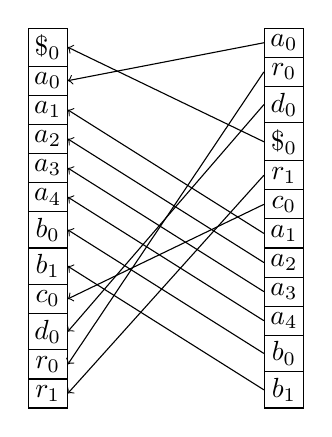
\begin{tikzpicture}
        \node[rectangle split, rectangle split parts=12,draw,inner sep=.5ex] (A) at (0,1)
        { 
            \(\$_0\)\nodepart{two}
            \(a_0\)\nodepart{three}
            \(a_1\)\nodepart{four}
            \(a_2\)\nodepart{five}
            \(a_3\)\nodepart{six}
            \(a_4\)\nodepart{seven}
            \(b_0\)\nodepart{eight}
            \(b_1\)\nodepart{nine}
            \(c_0\)\nodepart{ten}
            \(d_0\)\nodepart{eleven}
            \(r_0\)\nodepart{twelve}
            \(r_1\)\nodepart{thirteen}
            };
        
        \node[rectangle split, rectangle split parts=12,draw,inner sep=.5ex] (B) at (3,1)
        {   
            \(a_{0}\)\nodepart{two}
            \(r_0\)\nodepart{three}
            \(d_0\)\nodepart{four}
            \(\$_0\)\nodepart{five}
            \(r_1\)\nodepart{six}
            \(c_0\)\nodepart{seven}
            \(a_1\)\nodepart{eight}
            \(a_2\)\nodepart{nine}
            \(a_3\)\nodepart{ten}
            \(a_4\)\nodepart{eleven}
            \(b_0\)\nodepart{twelve}
            \(b_1\)\nodepart{thirteen}
            };
        %\draw[->] (B.four west) -- (A.four east);
        \draw[<-] (A.four east) -- (B.eight west);
        %\draw[->] (B.eight west) -- (A.eight east);
        \draw[<-] (A.eight east) -- (B.twelve west);
        %\draw[->] (B.twelve west) -- (A.twelve east);
        \draw[<-] (A.twelve east) -- (B.five west);
        %\draw[->] (B.five west) -- (A.five east);
        \draw[<-] (A.five east) -- (B.nine west);
        %\draw[->] (B.nine west) -- (A.nine east);
        \draw[<-] (A.nine east) -- (B.six west);
        %\draw[->] (B.six west) -- (A.six east);
        \draw[<-] (A.six east) -- (B.ten west);
        %\draw[->] (B.ten west) -- (A.ten east);
        \draw[<-] (A.ten east) -- (B.three west);
        %\draw[->] (B.three west) -- (A.three east);
        \draw[<-] (A.three east) -- (B.seven west);
        %\draw[->] (B.seven west) -- (A.seven east);
        \draw[<-] (A.seven east) -- (B.eleven west);
        %\draw[->] (B.eleven west) -- (A.eleven east);
        \draw[<-] (A.eleven east) -- (B.two west);
        %\draw[->] (B.two west) -- (A.two east);
        \draw[<-] (A.two east) -- (B.one west);
        %\draw[->] (B.one west) -- (A.one east);
        \draw[<-] (A.one east) -- (B.four west);
        %\node (C) [below=of A]{Matrix Class};
        %\node[below= .5cm of B,text width=2cm,align=center]{Double Matrix\\ Class};
    \end{tikzpicture}
    \caption{Visualization of the mapping \(T\). Identical characters are mapped according to their relative position, as expressed by the numbering of the characters. We note that the numbering is only for illustrative purposes.}
\end{figure}
With \(I=3\), 
\begin{align*}
    c_0 &= L[T^{0}[3]] & &= L[3] &= \$ \\
    c_1 &= L[T^{1}[3]] &= L[T[3]] &= L[0] &= a \\
    c_2 &= L[T^{2}[3]] &= L[T[0]] &= L[1] &= r \\
    c_3 &= L[T^{3}[3]] &= L[T[1]] &= L[10] &= b \\
    c_4 &= L[T^{4}[3]] &= L[T[10]] &= L[6] &= a \\
    c_5 &= L[T^{5}[3]] &= L[T[6]] &= L[2] &= d \\
    c_6 &= L[T^{6}[3]] &= L[T[2]] &= L[9] &= a \\
    c_7 &= L[T^{7}[3]] &= L[T[9]] &= L[5] &= c \\
    c_8 &= L[T^{8}[3]] &= L[T[5]] &= L[8] &= a \\
    c_9 &= L[T^{9}[3]] &= L[T[8]] &= L[4] &= r \\
    c_{10} &= L[T^{10}[3]] &= L[T[4]] &= L[11] &= b \\
    c_{11} &= L[T^{11}[3]] &= L[T[11]] &= L[7] &= a
\end{align*}
Which gives us the original string \(S="abracadabra\$"\), where the \(\$\) can be discarded.

\subsection{Move-to-front Encoding}\label{sectionMTF}
% TODO improve this
% TODO reference the papers of MTF

Burrows and Wheeler suggested the usage of Move-to-front (\texttt{MTF}) encoding after the \texttt{BWT}. \texttt{MTF} encoding is a reversible lossless encoder that does not change the size of the input, but further preprocesses it.
This is done to achieve a higher concentration of characters on our data, preparing it for Huffman encoding or arithmetic encoding. As previously mentioned, after the \texttt{BWT} step, we expect that similar characters will be grouped together. This means that there will contain segments with few diverse characters or even only contain identical characters. \texttt{MTF} encodes each of these segments of similar characters to a segment of low valued characters.
% TODO

\subsubsection{Encoding}
\texttt{MTF} maintains a list of frequently seen characters containing the alphabet. It encodes each character by replacing it with its index in this list, and then updates the list moving that character to the front of the list.
%\begin{algorithm}[H]
%    \caption{Move-to-front Encode}\label{alg:cap}
%    \begin{algorithmic}[1]
%        \Procedure{MTF\_Encode}{bytes}
%            \State \(\Sigma \gets [0, 1, 2, \dots , 255]\)
%            \For{i = 0 \dots bytes.length - 1}{
%                \State $code \gets$ \Sigma.index(bytes[i])
%                \State \(bytes[i] \gets code\)
%                \Sigma.remove(bytes[i])
 %               \Sigma.prepend(bytes[i])
%            }
%        \EndProcedure
%    \end{algorithmic}
%\end{algorithm}

We illustrate this with an example. Continuing from our example from the \texttt{BWT}, we wish to \texttt{MTF} encode the string \(L = "ardrcaaaabb"\). We initialize our alphabet list such that it contains the unique characters appearing in \(L\) sorted in alphabetical order \(\Sigma=[a, b, c, d, r]\).
The same initial characters list used when encoding is required for decoding, therefore it is usually implemented to be the same in the encoder/decoder implementation. 
Now we iterate through \(L\). For each character in \(L\), we replace it by the index in which it appears in the list. Then we pop that character from its position in the list and preprend it to the front of the list.
{
    \begin{align*}
        |ardrcaaaabb \quad \quad\quad [a, b, c, d, r] \\[-4pt]
        0|rdrcaaaabb \quad \quad\quad [a, b, c, d, r] \\[-4pt]
        04|drcaaaabb \quad \quad\quad [r, a, b, c, d] \\[-4pt]
        044|rcaaaabb \quad \quad\quad [d, r, a, b, c] \\[-4pt]
        0441|caaaabb \quad \quad\quad [r, d, a, b, c] \\[-4pt]
        04414|aaaabb \quad \quad\quad [c, r, d, a, b] \\[-4pt]
        044143|aaabb \quad \quad\quad [a, c, r, d, b] \\[-4pt]
        0441430|aabb \quad \quad\quad [a, c, r, d, b] \\[-4pt]
        04414300|abb \quad \quad\quad [a, c, r, d, b] \\[-4pt]
        044143000|bb \quad \quad\quad [a, c, r, d, b] \\[-4pt]
        0441430004|b \quad \quad\quad [b, a, c, r, d] \\[-4pt]
        04414300040| \quad \quad\quad [b, a, c, r, d]
    \end{align*}
}
The output of the \texttt{MTF} with input \(L = "ardrcaaaabb"\) is then \("04414300040"\). After the \texttt{BWT} step, the \texttt{MTF} encoder replaces segments containing similar characters with low numbers since the characters that were recently seen are located at the front of the list. 
For runs of identical characters, the \texttt{MTF} step replaces these with a specific index, followed by many zeros. For a run of identical characters, only the first character needs to have a non-zero value, and then the rest will become zero values.
After this step, if the \texttt{BWT} was successful, our data will contain a high concentration of character frequencies.
% This algorithm takes O(nk), where n is the size of the input and k is a constant, usually 256.


\subsubsection{Effect on Data}
We test the \texttt{MTF} transform on the output of the \texttt{BWT} on the files from the Silesia Corpus. We use a specific byte alphabet that covers in order: 96-127 (lowercase), 64-95 (uppercase), 32-63 then 0-31 (punctuation/number) and finally non-ascii numbers of 128-255. This is written as 
\[
    \Sigma = [96, \dots , 127, 64, \dots , 95, 32 \dots, 63, 0 \dots 31, 128 \dots 255].
\] 
We graph the byte frequencies after the transform. The assumption is that after the \texttt{MTF} the frequency of bytes will be greatly skewed towards the lower valued bytes, such that more than half of the data consists of only the first few bytes.
\begin{figure}[H]
    \centering
    \includegraphics[width=\textwidth]{images/mtfGraphFreq.png}
    \caption{Stacked bar chart showing byte frequencies percentage over the different files in the Silesia Corpus. Each bar in the stacked bars is the percentage of frequency of a byte, where there are 256 bytes in total. The first bar from the bottom is 0, second is 1, etc.}
    \label{MTFFreq}
\end{figure}
For some files such as \texttt{dickens}, \texttt{xml} and \texttt{nci}, more than 90\% of the bytes are the first 10 bytes. \texttt{nci} shows an extreme example where \texttt{BWT} has very effectively grouped the characters up in runs, since the 0-byte consists of over 90\% of the \texttt{MTF}. A less extreme example is for the file \texttt{dickens}. Here, there are perhaps fewer and/or shorter runs in the output of the \texttt{BWT}, but it is observable that there are few different bytes that appear next to each other.
\begin{figure}[H]
    \centering
    \includegraphics[width=\textwidth]{images/saoCharFreq.png}
    \caption{Frequencies of the bytes \(0 \dots 255\) in the \texttt{sao} in the Silesia Corpus before (left) and after (right) using \texttt{BWT} and \texttt{MTF}. Note that the y-axis is logarithmic.}
\end{figure}
Although the characters in the original file \texttt{sao} consists of all bytes of \(0 \dots 255\), it contains some characters with similar right-context, since after using \texttt{BWT} and \texttt{MTF} the byte frequencies are highly skewed towards the smaller byte values.

% TODO we can initialize the alphabet better so it has more zeros

\subsubsection{Decoding}
Decoding the \texttt{MTF} requires a similar procedure to its encoding. This time, instead of finding the index of the specific character, we instead index into the list using the number we are at. We then again move than character to the front of the list.

We illustrate using our \texttt{MTF} encoded example of \("04414300040"\). We initialize the same alphabet list that we used for the encoding \(\Sigma = [a, b, c, d, r]\). Each number in the encoded string represents the index of the original character in the list. So we replace each number with the character in that position in the list and move that character to the front of the list.
{
    \begin{align*}
        |04414300040 \quad \quad\quad [a, b, c, d, r] \\[-4pt]
        a|4414300040 \quad \quad\quad [a, b, c, d, r] \\[-4pt]
        ar|414300040 \quad \quad\quad [r, a, b, c, d] \\[-4pt]
        ard|14300040 \quad \quad\quad [d, r, a, b, c] \\[-4pt]
        ardr|4300040 \quad \quad\quad [r, d, a, b, c] \\[-4pt]
        ardrc|300040 \quad \quad\quad [c, r, d, a, b] \\[-4pt]
        ardrca|00040 \quad \quad\quad [a, c, r, d, b] \\[-4pt]
        ardrcaa|0040 \quad \quad\quad [a, c, r, d, b] \\[-4pt]
        ardrcaaa|040 \quad \quad\quad [a, c, r, d, b] \\[-4pt]
        ardrcaaaa|40 \quad \quad\quad [a, c, r, d, b] \\[-4pt]
        ardrcaaaab|0 \quad \quad\quad [b, a, c, r, d] \\[-4pt]
        ardrcaaaabb| \quad \quad\quad [b, a, c, r, d]
    \end{align*}
}
Which gives us our original decoded string \(S="ardrcaaaabb"\) from the encoded string \("04414300040"\).


\subsection{Huffman Encoding}\label{sectionHuff}
Huffman Encoding is a type of variable-length encoding technique that is widely used in lossless compression. The Huffman algorithm takes a set of characters and their number of occurrences in the data, known as the character frequencies. It then creates a mapping where it maps each character to a prefix-free code. Here each code has variable length and is represented in binary for file compression.
This is useful after the \texttt{MTF} step since we expect that the data consists of skewed frequencies of data, where the data consists of relatively few different characters. This type of data is good to encode using Huffman encoding since we can encode the very frequent characters using the shortest bit-codes while neglecting the less frequent characters and giving them the longer codes. 
% TODO: side 429 i Cormen

\subsubsection{Encoding}
The Huffman algorithm is a greedy algorithm that takes a set of characters and their frequencies and constructs a Huffman tree that is a binary tree. The leaves of the Huffman tree are characters, and the path from the root to the leaves describes the bit code for the specific character in the leaf. 
Performing the Huffman algorithm on \(n\) characters, we initially have \(n\) trees, each only containing the root node, which contains the specific character and its frequency in the data. 
The algorithm then repeatedly greedily combines the two trees with the lowest frequency merging them into one tree by adding their root node as children to a new parent node, where the new root node has a frequency the sum of its two new children. This procedure requires \(n - 1\) merges in total, which at the end of the merges leaves one remaining tree, which is the Huffman tree.
The Huffman tree can then be traversed from the root to the leaves to retrieve the code for the character on that leaf. For each node going to the left child we write a 0-bit and going to the right child we write a 1-bit, until a leaf is reached.

After encoding each byte with its bitcode from the Huffman tree, we may end up with a number of bits not a multiple of 8. In practice, since a computer file is always stored in bytes, the amount of bits written need to be a multiple of 8. If we finish encoding and this is not the case, we can pad the remaining unfinished byte with 0-bits.

\subsubsection{Decoding}\label{SectionHuffmanDecoding}
In order to decode we require the exact same Huffman tree that was used for encoding. Once we have that same tree, the procedure then consists of starting from the root, continuously reading the bits of the encoded data, and traversing the tree until reaching a leaf. When we reach a leaf we write the symbol associated with that leaf and return to the root, continuing reading the bits.

In order to retrieve the same Huffman tree we used for encoding, there are several techniques that can be used depending on the type of data. The naive technique is to simply write the byte frequencies used to create the Huffman tree to the start of the compressed file. When we decode, we start by reading the frequencies, then creating the Huffman tree, and then following the normal decoding procedure. This is however not always used in practice since it requires a lot of overhead cost. If we assume that the maximum frequency of a character can be written using 4 bytes, then we need \(4 \cdot 256 = 1024\) bytes of overhead.

Another complication is to know when to stop reading the last byte of the encoded data. Since we possibly padded the last byte with 0-bits, it may be ambiguous whether when exactly we should stop reading the last byte.
One way to know when we have reached the end is to write the amount of characters that were encoded so we know to stop when we have read the same amount of characters during decoding. Another way is to add a unique special \texttt{EOF} character to the end of the file when encoding. This character is also encoded with its own code when Huffman encoding and will possibly have one of the longest codes since it has a frequency of only one. When decoding, if read this special we know to stop reading further bits.

The specific technique for both these problems depends on the specific compressor and decompressor implementations. The research report by Burrows and Wheeler does not describe how these two problems are handled in their algorithm. We will in \cref{CannonicalHuffmanTree} describe how \texttt{bzip2} handles these two complications.


% Burrows and Wheeler mention tThe implementation by Burrows and Wheeler

\section{bzip2}\label{sec:BZIP2}
\texttt{bzip2} is a general-purpose lossless file compressor. The first version released by Julian Seward in 1996, with version 1.0 released in 2000. As previously mentioned, it belongs to the class of Burrows--Wheeler based compressors, since it uses the \texttt{BWT} at core of its compression.

\texttt{bzip2} combines five layers of compression techniques and algorithms. These layers are Run-length encoding \texttt{RLE 1}, \texttt{BWT}, \texttt{MTF}, \texttt{RLE 2} and Huffman encoding using multiple Huffman trees.

\subsection{Run-length Encoding}\label{BZIP2RLE}
Run-length Encoding (\texttt{RLE}) is a lossless data encoder that encodes runs of identical characters. A sequence of identical characters is encoded by an identifier, identifying what specific character it contains and the amount of them. This encoding can be applied to any type of data that contains sequences of identically repeating characters.

We show an example of this encoding. Assume that we wish to encode \(WaaaaabbbbcaaaaW\) using \texttt{RLE}. We know that the string can be represented as being a string consisting of respectively 5 \(a\)'s, 4 \(b\)'s, 1 \(c\), and 4 \(a\)'s. We can write this encoding as the following
\[
aaaaabbbbcaaaa \rightarrow 5a4bc4a.
\]
% TODO .. what?
While this encoding step reduces the size of the message, it introduces new characters since it needs to identify the number of characters in the encoded runs.
\\

\texttt{bzip2} uses \texttt{RLE} twice, we will denote these two separatly as \texttt{RLE 1} and \texttt{RLE 2}. 
\texttt{RLE 1} is the first compression encoding technique used in the compressor. It was originally included as a pre-processer to the sorting in the \texttt{BWT} step in order to avoid pathological inputs. It has however since been described in the \texttt{bzip2} manual by the author to be "entirely irrelevant". We will therefore not describe it in this report. % TODO: CITE "entirely irrelevant"
The second \texttt{RLE} step, \texttt{RLE 2} is used after the \texttt{MTF} step. This is used to take advantage of the output of the \texttt{MTF} step. Since as previously mentioned, from the output of the \texttt{MTF} step we can expect our data to contain some runs of zeros. The \texttt{RLE} will remove these consecutive zeros and instead write the amount appearing consecutively in binary representation using two new characters \texttt{RA} and \texttt{RB}. To illustrate this, consider an array containing a valid output from the \texttt{MTF} step: for example \(S = [0, 4, 4, 1, 4, 3, 0, 0, 0, 4, 0]\), we can represent the number of zeros in the runs in binary representation using the two new characters \texttt{RA} and \texttt{RB}.
\[
    [0, 4, 4, 1, 4, 3, 0, 0, 0, 4, 0] \longrightarrow [\texttt{RA}, 4, 4, 1, 4, 3, \texttt{RA}, \texttt{RA}, 4, \texttt{RA}],
\]
where \texttt{RA} represents 1 zero and \texttt{RA} \texttt{RA} represents 3 zeros. As per binary encoding illustrated with the following table
\begin{table}[H]
    \centering
    \begin{tabular}{|c|c|}
        \hline
        1 & \texttt{RA} \\ \hline
        2 & \texttt{RB} \\ \hline
        3 & \texttt{RA} \texttt{RA} \\ \hline
        4 & \texttt{RB} \texttt{RA} \\ \hline
        5 & \texttt{RA} \texttt{RB} \\ \hline
        6 & \texttt{RB} \texttt{RB} \\ \hline
        7 & \texttt{RA} \texttt{RA} \texttt{RA} \\ \hline
        8 & \texttt{RB} \texttt{RA} \texttt{RA} \\ \hline
    \end{tabular}
    \quad
    \begin{tabular}{|c|c|}
        \hline
        9 & \texttt{RA} \texttt{RB} \texttt{RA} \\ \hline
        10 & \texttt{RB} \texttt{RB} \texttt{RA} \\ \hline
        11 & \texttt{RA} \texttt{RA} \texttt{RB} \\ \hline
        12 & \texttt{RB} \texttt{RA} \texttt{RB} \\ \hline
        13 & \texttt{RA} \texttt{RB} \texttt{RB} \\ \hline
        14 & \texttt{RB} \texttt{RB} \texttt{RB} \\ \hline
        15 & \texttt{RA} \texttt{RA} \texttt{RA} \texttt{RA} \\ \hline
        16 & \texttt{RB} \texttt{RA} \texttt{RA} \texttt{RA} \\ \hline
    \end{tabular}
    \caption{Binary encoding of the first 16 consecutive amounts of the 'zero' character using the two new characters \texttt{RA} and \texttt{RB}. We note that \texttt{bzip2} encodes with bit significance in reverse order, where the least significant bit is the first bit from the left.}
    \label{tab:my_label}
\end{table}
Our binary counting starts from one since we know that the appearance of either a \texttt{RA} or a \texttt{RB} character represents the occurrence of at least one zero character in that location. In this step, there is also no need to write what character is being encoded, since it by definition only encodes the zero character.

After having introduced the two new characters, we will possibly have 258 characters in total. After this step however, our data will not contain any zero-byte characters, meaning our data will contain at most 257 characters, which are these following characters.
\begin{center}
    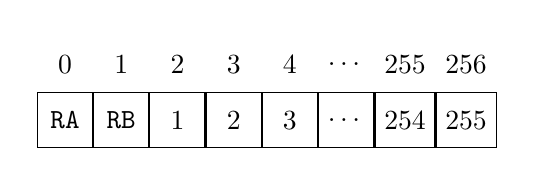
\begin{tikzpicture}
        \matrix (m) [matrix of nodes,
                     nodes={draw, minimum size=7mm,anchor=center},
                     nodes in empty cells, minimum height = 1cm,
                     row 1/.style={nodes={draw=none}},]
        {
          0 & 1 & 2 & 3 & 4 & \dots & 255 & 256  \\
          \texttt{RA} & \texttt{RB} & 1 & 2 & 3 & \dots & 254 & 255 \\
        };
    \end{tikzpicture}
\end{center}
After the \texttt{RLE 2} step, to prepare for the next step which is Huffman encoding, we add a new EOF character at the end of the data to represent the end of the data. Giving us the following 258 characters
\begin{center}
    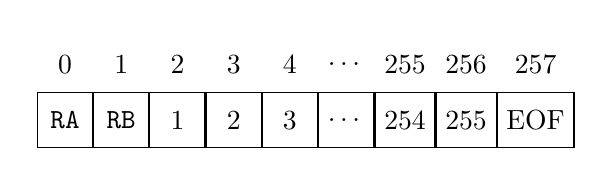
\begin{tikzpicture}
        \matrix (m) [matrix of nodes,
                     nodes={draw, minimum size=7mm,anchor=center},
                     nodes in empty cells, minimum height = 1cm,
                     row 1/.style={nodes={draw=none}},]
        {
          0 & 1 & 2 & 3 & 4 & \dots & 255 & 256 & 257  \\
          \texttt{RA} & \texttt{RB} & 1 & 2 & 3 & \dots & 254 & 255 & EOF \\
        };
    \end{tikzpicture}
\end{center}
We will explain the reason for this new character in the next section.

% Successor to bzip1 because of patent

\subsection{Multiple Huffman Trees}
As examined in \cref{sectionHuff}, Huffman encoding guarantees symbol-code optimality for the entire data, but is not necessarily optimal for individual segments of the data. For this reason, the \texttt{bzip2} compressor uses multiple Huffman trees which generally yields better compression for large data. The amount of trees it uses is dependent on the size of the data and is between 2 and 6 (inclusive). Although is most commonly 6 when used to encode reasonably sized data.

Each segment of 50 characters in the data is encoded using the specific Huffman tree that is cheapest for that segment. We will explain how the Huffman trees are generated and then improved in the following sections. We define \(k\) to be the amount of Huffman trees used, where \(2 \leq k \leq 6\).

\subsubsection{Huffman Trees Initialization}\label{HuffmanTreeInit}
% TODO: Does below make sense?
The first step is to partition the characters into \(k\) continuous intervals such that each interval makes up approximately \(\frac{1}{k} \cdot 100\%\) of the character frequencies.

For example, if we assume we will have \(k = 6\) Huffman trees, then each character-interval must consist of approximately \(16\%\) of the data. 
\begin{table}[H]
    \centering
    \begin{tabular}{|c|c|c|}
        \hline
        idx & Character intervals & Coverage \\\hline
        0 & 0 \dots 4 & 19.7\% \\ \hline
        1 & 5 \dots 14 & 15.7\% \\ \hline
        2 & 15 \dots 48 & 16.3\% \\ \hline
        3 & 49 \dots 108 & 15.9\% \\ \hline
        4 & 109 \dots 181 & 16.4\% \\ \hline
        5 & 182 \dots 257 & 16.0\% \\  \hline
    \end{tabular}
    \caption{Example of the partitions on the character-intervals for k = 6. These are the \texttt{bzip2} partitions on the first block when compressing the file \texttt{sao} from the Silesia Corpus. \texttt{bzip2 -k -vvv silesia/sao}.}
    \label{table:tableIntervalPartition}
\end{table}
A simple method to calculate these character intervals is to continuously add a new character to the current interval until that interval covers \(\frac{1}{k} \cdot 100\%\) of the character frequencies, which after then move on to the next interval until all the data is covered. Although this method works, it gives each interval except the last one \(\geq \frac{1}{k} \cdot 100\%\), which means the last interval may be greatly unsaturated, potentially covering much less than the optimal percentage. 
The implementation in \texttt{bzip2} fixes this issue by removing the last character in the odd numbered intervals, except for the last interval. This results in the even numbered trees to cover more than or equal the optimal amount, and the odd numbered trees (except for the last one) to cover less than or equal the optimal percentage. As can be seen in the interval coverages in \cref{table:tableIntervalPartition}.

\subsubsection{Huffman Trees Iterative Improvement}\label{HuffmanIterativeImprovementSection}
The character intervals generated in the previous \cref{HuffmanTreeInit} are used to generate the Huffman trees. This is done by finding the cheapest interval for each of the 50-character segments separately. This will be the interval in which most characters in that segment are in. After these segments are partitioned into the intervals, the Huffman trees are computed from the character frequencies from the segment partitions.

Computing the Huffman trees gives us a new way to calculate the segment partitions, we can calculate the cheapest Huffman tree on the specific segment according to the code lengths on the character frequencies of that segment. \texttt{bzip2} iterates \(\texttt{BZ\_N\_ITERS} = 4\) times (by default), to improve the Huffman trees, where each time we compute the segment partitions, giving the cheapest Huffman tree the partition in accordance to its code lengths. We then recompute the Huffman trees according to these partitions. This gives a way for each Huffman tree to specialize in specific segments of the data, which are relatively similar in their symbol frequencies.

After the last iteration we can recalculate the current best segment partitions for the Huffman trees. This yields the specific Huffman tree to encode the segments with. For each segment there is identified, in zero-terminated unary encoding, which Huffman tree out of \(k\) is used to encode that segment.
\[
    0: 0 \quad 1: 10 \quad 2: 110 \quad 3: 1110 \quad 4: 11110 \quad 5: 111110
\]


\subsubsection{Canonical Huffman Trees}\label{CannonicalHuffmanTree}
When we decode Huffman encoding we need to use the same tree(s) used for encoding. Instead of the naive method of writing the frequencies of each byte in the header of the encoded file, as mentioned in \cref{SectionHuffmanDecoding}, \texttt{bzip2} instead uses the code lengths of each character. This however introduces ambiguity since codes of the same length can be different. This is why \texttt{bzip2} uses canonical Huffman trees that are generated from the code lengths. For encoding, \texttt{bzip2} uses the Huffman algorithm to compute the optimal code lengths. From those code lengths it generates another Huffman tree that is canonical. In this way, given the same code lengths when encoding and decoding, the canonical Huffman tree will be same.
Given an array \(code\_length[0 \dots 257]\) that contains code lengths that are valid for a binary tree, where the code length of character \(c\) is \(code\_length[c]\), we can generate the codes of the canonical Huffman tree as follows.
\begin{lstlisting}[language=Python, caption={We generate the codes that have shortest code lengths first. Line 7 changes the code by adding the value 1, for characters with the same length, and then another time before the length changes, to have prefix-free codes. We then bit shift by 1 since we descent one step down the Huffman tree (line 8).}]
    code = 0
    codes = [None] * 258
    for l in range(len_min, len_max + 1):
        for c in range(0, CHAR_MAX + 1):
            if (l == code_length[c]):
                codes[c] = code
                code += 1
        code = code << 1;
\end{lstlisting}
This generates consistent Huffman codes given valid Huffman code lengths. The Huffman tree will be skewed as the shortest codes will be aligned to the left, and the longest codes aligned to the right.

Instead of writing all Huffman tree code lengths in the header, \texttt{bzip2} only writes the code length of characters that have non-zero frequency. For the decompressor implementation to know which code lengths are encoded, the compressor writes a 2-level character map using up to \(16+256=272\) bits. The first level is 16 bits which denote, if there is a non-zero frequency code length for characters with 16 size interval. For example if the first 16 bits are 1000000100010000, then we know that next level character map contains \(3 \cdot 16 = 48\) bits, which denote whether a code length is written. The intervals of these characters are \(2 \dots 18\), \(115 \dots 130\) and \(163 \dots 179\).
\texttt{bzip2} assumes that there is always a code length for the character 0 and 1, which are the \texttt{RLE} special characters \texttt{RA} and \texttt{RB}.

The code lengths are then encoded using delta encoding, which starts from an initial code length with 5 bits encoding the initial length of the \texttt{RA} character. For the delta encoding, reading the continuously, reading bits 10 we increment the current code length by, and reading a 11 we decrement the code length by 1. Reading a 0 outside of these means our current code length is the length for this character, and we can move to the next character.

We have devised a more efficient delta encoding, which saves cost at every step instead of using 10 and 11, and then 0 as termination, as \texttt{bzip2} uses. Our proposal is using an initial 1 which shows that the difference in code length is non-zero. Then using a 0 for positive code length difference and a 1 for negative code length difference. And then encoding using unary encoding until we see a 0.
We can compare these two delta encoding techniques according to their cost in bits

\begin{table}[H]
    \centering
    \begin{tabular}{|c|c|c|c|c|}
        \hline
        & \multicolumn{2}{c|}{\(bzip2\)} & \multicolumn{2}{c|}{Proposed method} \\ \hline
        Difference & Coding & Cost & Coding & Cost \\ \hline
        0 & 0 & 1 & 0 & 1  \\ \hline
        \(+1\) & 100 & 3 & 100 & 3 \\ \hline
        \(-1\) & 110 & 3 & 110 & 3 \\ \hline
        \(+2\) & 10100 & 5 & 1010 & 4 \\ \hline
        \(-2\) & 11110 & 5 & 1110 & 4 \\ \hline
        \(+3\) & 1010100 & 7 & 10110 & 5 \\ \hline
        \(-3\) & 1111110 & 7 & 11110 & 5 \\ \hline
        \(+4\) & 101010100 & 9 & 101110 & 6 \\ \hline
        \(-4\) & 111111110 & 9 & 111110 & 6 \\ \hline
    \end{tabular}
    \caption{Our proposed cheaper delta encoding for encoding the code lengths of the Huffman trees as opposed to the method \texttt{bzip2} uses.}
    \label{tab:my_label}
\end{table}
For all delta encodings, our values are cheaper.


\section{Experiments}\label{sec:EXPERIMENTS}
\subsection{Experimental Setup}
Our experimental setup is an attempted recreation of the main algorithms used from \texttt{bzip2} in \texttt{Java}, with some justified exclusions. We have excluded the usage of the first layer which is \texttt{RLE 1} due to its irrelevance. We instead perform \texttt{BWT} directly on the data. Our implementation also does not use block sizes of 900 kB, and so compresses any size without dividing it into smaller blocks.

%We implement the methods presented in 3 to compare compression ratio.
% The focus is compression ratio, not speed
\subsection{Run-length Encoding (RLE 2)}
Although not mentioned by name in the original report by Burrows and Wheeler, they use in their implementation a \texttt{RLE} type scheme, which uses a Huffman tree to write the binary codes for the different lengths of runs, instead of simply using binary encoding as \texttt{bzip2} does.
As mentioned in \cref{BZIP2RLE}, \texttt{bzip2} uses \texttt{RLE} which replaces the runs of zeros with binary encoding using two new characters that indicates the length of the run. The size of the data after this step will often be shorter, but never longer, with the cost of introducing two new characters. 

We can measure the difference in compression ratio when using \texttt{RLE 2}.
\begin{figure}[H]
    \centering
    \includegraphics[width=\textwidth]{images/RLEWithWithout.png}
    \caption{Bar chart showing showing the sizes of the encoded files in bytes when using \texttt{RLE} versus when not using it.}
\end{figure}
It is reasonable to assume previous results, from \cref{avgRunsLengthFigure} and \cref{MTFFreq} that the \texttt{RLE 2} step excels when the data after the \texttt{BWT} has a high average run length. This is not necessarily equivalent to the data containing many zeros after the \texttt{MTF}. This is the case since the data can contain a mixture between the absolute number of runs and the average length of those runs, and these are not necessarily equivalent for \texttt{RLE}, since it excels when the data after the \texttt{BWT} contains a high average run length.

In any case though, there seems to be no reasonable reason to exclude this step, even though it introduces two new characters it shows promising results.

Another method which could have been deployed is to Huffman encode the binary encodings representing the run lengths. This was suggested in the original paper by Burrows and Wheeler. The assumption is that this is more efficient if the runs in the \texttt{BWT} data tends to appear in runs of same length, for example if it contains more runs of length 5 than it contains runs of length 3, then the run of length 5 can be encoded in binary using fewer bits than the run of length 3.

\subsection{Huffman Trees Selectors Encoding}
We wish to compare how often the different Huffman trees are used in the 50 character sized segments. After the iterations which improve the Huffman tree, we have the segment partition which defines which Huffman tree is used at each partition. We count the number of partitions that belong to each tree. The assumption here is that first Huffman tree will have the greatest share of segments since it always contains the 0-byte in its initial interval. With this however, the last Huffman tree may also have a large share of segments, since it on average contains the largest range of different characters in its interval.
\begin{figure}[H]
    \centering
    \includegraphics[width=\textwidth]{images/Selectors.png}
    \caption{Stacked bar chart showing the amount of segments each Huffman tree has in terms of the total number of segments in the data.}
\end{figure}
Which gives the following Huffman tree selector percentages
\begin{table}[H]
    \centering
    \begin{tabular}{|c|c|c|}
         \hline
         Selector & Unweighted \% & Weighted \% \\ \hline
            0 &	19.09\%	 & 20.22\% \\ \hline
            1 &	14.43\% &	14.00\% \\ \hline
            2 &	12.65\% &	13.21\% \\ \hline
            3 &	15.61\%	& 14.09\% \\ \hline
            4 &	21.08\% &	17.92\% \\ \hline
            5 &	17.13\% &	20.57\% \\ \hline
    \end{tabular}
    \caption{Huffman tree segment selectors, showing the average selectors both unweighted and weighted, where weighted denotes a weighted average where the file size is the weight.}
\end{table}
As can be seen, the first and last Huffman trees are in average used 40\% of the time. In this example the last Huffman tree is used more than the first Huffman tree. Since \texttt{bzip2} uses unary encoding to encode which Huffman tree it uses. We can calculate the number of bits that are used on average on this, given the our data.
\[
    0.202 + 2 \cdot 0.14 + 3 \cdot 0.132 + 4 \cdot 0.141 + 5 \cdot 0.179 + 6 \cdot 0.206 = 3.573 \text{ bits}
\]
A different way these selectors can be encoded is using binary encoding. For 6 Huffman trees we require 3 bits per selector instead of the 3.573 bits we have seen in our test data. This for our specific examples is more efficient encoding and saves us 0.573 bits on average for each selector. This is however not the only reason reason to change to binary encoding, and we will in the following section see how this can further be taken advantage of.

\subsection{Huffman Trees Amount}\label{HuffmanTreesCount}
The number of Huffman trees \texttt{bzip2} uses is from 2 to 6. This preset cap of 6 may make sense when encoding in chunks of 900 kB and when using unary encoding to encode the selectors. From last section we suggested using binary encoding instead of unary encoding for the Huffman tree segment selectors. This uses a variable amount of bits (which is dependant on the amount of trees used) per selector instead of the unary encoding which \texttt{bzip2} uses.
This allows us to have up to 8 Huffman trees using 3 bits, and further up to 16 Huffman trees using 4 bits, in fact when we have \(k\) Huffman trees we need \(\lceil\log_2{(k)}\rceil\) bits to encode the selectors.
Because of this, our assumption is that it is most reasonable to use an amount of Huffman trees that is a power of two. Since there otherwise is redundancy in our binary encoding of the selectors.
This of course assumes that the cost of the overhead of the Huffman trees can be neglected for large enough data.

We test this using Huffman trees ranging from 1 to 16.
\begin{figure}[H]
    \centering
    \includegraphics[width=\textwidth]{images/HuffmanTreesCount.png}
    \caption{Encoded file size as percentage of the original file size (y) using different number of Huffman trees (x).}
\end{figure}
It can be observed that using two Huffman trees instead of one leads to better compression ratio for all test files.
However, our assumption that using Huffman trees up to a power of 2 should always lead to better compression, is not necessarily what we observe. For the file \texttt{osdb}, surprisingly, using 13 Huffman trees leads to better compression than using 16, and this is large difference is not due to the overhead of storing the code lengths for the Huffman tree.
This means that the steps \texttt{bzip2} uses to generate the Huffman trees (described in \cref{HuffmanTreeInit} and \cref{HuffmanIterativeImprovementSection}) does not lead to optimal partitions of the segments to be encoded each with their own Huffman tree.


\subsection{Huffman Trees Improvement Iterations}
As described previously, \texttt{bzip2} iterates 4 times (by default) to improve the segment partitions to improve the Huffman trees. If we assume that more iterations will mostly lead to better compression and never lead to worse compression, then the specific number of iterations seems to be a compression ratio / time trade off, until we hit a limit.
Although as tested in the previous section, the method \texttt{bzip2} uses to generate the Huffman tree does not seem to be optimal, therefor it is not strictly obvious that more iterations can't lead to worse compression ratio. 

We test the compression ratio when iterating from a range of 1 to 7.
\begin{figure}[H]
    \centering
    \includegraphics[width=\textwidth]{images/treesIterationsCount.png}
    \caption{Compression as percentage of original file (y) on a different number of improvement iterations (x).}
\end{figure}
Although the partitions are not necessarily global optimum, further iterations of the Huffman trees seems to only ever improve compression. This supports the case that the initial Huffman trees, and then further iterations of improvement of those Huffman trees leads to a local minimum, and not necessarily a global minimum. The improvement iterations just get deeper in the local minima that the initial Huffman trees are at.

Improving this means we would need to improve the initialization of the Huffman trees, to something other than partitions on segments depending on the interval of characters on their frequency.

\subsection{Huffman Encoding Segments Size}
As previously mentioned, \texttt{bzip2} encodes each 50 characters using a specific Huffman tree of up to \(k=6\) total different Huffman trees. Decreasing this size of 50 characters means that the partitions can be more specialized to each Huffman tree, with the trade off of having to omit more bits to signal switching Huffman tree. If we have our block size at \(h\), which is default at 50, and \(n\) total characters we wish to encode using the \(k\) Huffman trees, we need a total of
\[
    \frac{n}{h} \cdot \lceil\log_2{(k)}\rceil \ \text{bits}
\]
to encode the Huffman segment selectors. This gives us a trade-off where we can use smaller or larger segment sizes, and therefor achieve more specialized partitions while using more bits to encode the segment selectors.

We can test the compression ratio in terms of using different sizes of these segments.
\begin{figure}[H]
    \centering
    \includegraphics[width=\textwidth]{images/HuffmanTreeBlockSizes.png}
    \caption{Compression as percentage of original file (y) on different block sizes (x). The block sizes tested range from 30 to 2000.}
\end{figure}
The optimal size of the segment seems to highly depend on what data we are compressing. For some files like \texttt{sao}, the optimal segment size is 100 or 200. For others like \texttt{xml}, we can achieve good compression using a range from 30-100, or 1000. There does not seem to be necessarily one one right optimal size value, but there can be multiple.

The compression achieved in these tests is of course highly dependant on the algorithms used to generate and improve the \(k\) Huffman trees.
An idea would be to use the same iteration process that \texttt{bzip2} uses, but for each \(m \geq 1\) improve iterations we decrease the segment size. This allows the Huffman trees to start from large segments and then slowly adapt and improve to fit smaller segments.




\section{Conclusion}
In this paper we have described the \texttt{BWT} which lies at the core of the \texttt{bzip2} compressor. We have described how to perform the \texttt{BWT} conceptually, how to reverse it and how to do it efficiently. We have further described other compression techniques \texttt{bzip2} uses, among these being \texttt{MTF}, \texttt{RLE} and then Huffman encoding using multiple Huffman trees. We have described how they work in theory, why they are effective at compressing data together, and the way \texttt{bzip2} has implemented them.

We have in depth analyzed the usage of multiple Huffman trees for Huffman encoding. We have experimented using different values than the hardcoded values used in \texttt{bzip2}. We have tested changing the values on the amount of Huffman trees, the size of the Huffman encoding segments and the amount of iterations to improve the Huffman trees.
For the different number of Huffman trees we have tested up to using 16 Huffman trees instead of the preset hardcoded cap of 6 Huffman trees used in \texttt{bzip2}. We have also tested the cost of encoding using multiple Huffman trees, where we encode both the code lengths and the selectors. Here we have proposed two methods which in our tests cases prove to be cheaper than the methods used in \texttt{bzip2}. From using more than 6 Huffman trees we have concluded that the algorithm \texttt{bzip2} uses to initialize and improve the Huffman trees does not necessarily lead to a global optimal, but instead a local optimal.

For future research, we could address the issue of initializing and improving the Huffman trees in order to compute the best segment partitions to be encoded using the multiple Huffman trees.


\newpage
\printbibliography %Prints bibliography

\newpage


\appendix

\end{document}
